\documentclass[12pt]{article}
\usepackage{amsmath}
\usepackage{amssymb}
\usepackage{tikz}
\usepackage{multirow}

\usepackage{graphicx} 
\usepackage{float} 

\begin{document}

$Email: LE000288@umn.edu$\\

$ID:5674954$\\

$\textbf{Problem 1}$\\

$\textbf{1}$\\

By using shape method, there are 3333 records in the dataset.\\

$\textbf{2}$\\

There are 21 features. They are 'state', 'account length', 'area code', 'phone number', 'international plan', 'voice mail plan', 'number vmail messages', 'total day minutes', 'total day calls', 'total day charge', 'total eve minutes', 'total eve calls', 'total eve charge', 'total night minutes', 'total night calls', 'total night charge', 'total intl minutes', 'total intl calls', 'total intl charge', 'customer service calls' and 'churn'.\\

'state' : Discrete\\
'account length': Discrete\\
'area code': Discrete\\
'phone number': Discrete\\
'international plan': Binary\\
'voice mail plan': Binary\\
'number vmail messages': Discrete\\
'total day minutes': Continuous\\
'total day calls': Discrete\\
'total day charge': Continuous\\
'total eve minutes': Continuous\\
'total eve calls': Discrete\\
'total eve charge': Continuous\\
'total night minutes': Continuous\\
'total night calls': Discrete\\
'total night charge': Continuous\\
'total intl minutes': Continuous\\
'total intl calls': Discrete\\
'total intl charge': Continuous\\
'customer service calls' and 'churn': Discrete\\

$\textbf{3}$\\

'account length', 'area code 'and 'phone number' are irrelevant. They are all nominal attributes. \\

$\textbf{4}$\\

By using info() method, we can find that there is no missing value.\\
\newpage
$\textbf{5}$\\

Table is above.\\

\begin{table}
\begin{tabular}{llllll}
                    & Average & Median & Maximum & Minimum & Std   \\
Total day minutes   & 179.775 & 179.4  & 350.8   & 0.00    & 54.47 \\
Total day charge    & 30.56   & 30.5   & 59.64   & 0.00    & 9.26  \\
Total eve minutes   & 200.98  & 201.4  & 363.7   & 0.00    & 50.71 \\
Total eve charge    & 17.08   & 17.12  & 30.91   & 0.00    & 4.31  \\
Total night minutes & 200.87  & 201.2  & 395.00  & 23.2    & 50.57 \\
Total night charge  & 9.04    & 9.05   & 17.77   & 1.04    & 2.27  \\
Total intl minutes  & 10.24   & 10.3   & 20.00   & 0.00    & 2.79  \\
Total intl charge   & 2.76    & 2.78   & 5.40    & 0.00    & 0.75 
\end{tabular}
\end{table}

$\textbf{6}$\\

The average number of customer service calls made by a customer to the company is 1.56.\\

$\textbf{7}$\\

Data comes from 51 states.\\

$\textbf{8}$\\

For "Churn" feature:\\

False    2850
True      483
Name: churn, dtype: int64\\

False samples are much more than True samples. Thus, this feature is skewed.\\

$\textbf{9}$\\

Highest ”total day charge” encountered by the customer:59.64\\

Lowest ”total day charge” encountered by the customer:0.00\\

When we sort the 'total day charge' in the descending order, we found that the top 10 customers all churning the company.
When we sort the 'total day charge' in the ascending order, we found that the 9 of the top 10 customers staying with the company. We may assume that the customers who pay high total day charge would more likely churn the company and the customers who pay low total day charge would more likely stay with the company.\\

$\textbf{10}$\\

The average number of customer service calls made by the user who has churned out of the company: 2.23.\\

The average number of customer service calls made by the user who is still with the company: 1.45.\\

The average number of customer service calls made by the user who has churned out of the company is larger than that of customer service calls made by the user who is still with the company.\\

$\textbf{11}$\\

By comparing the average values of numerical features for churned and non-churned users, we can find that the churned users have higher average 'total day minutes','total eve minutes ','customer service calls','many service calls ' than those of the non-churned users. The churned users spend more time on the calls and more customer service calls than those of the non-churned users. So the strategy would be improve the quality of the connection for the call, improve the quality of service and lower the calling price when the user call more.\\


$\textbf{12}$\\

\begin{figure}[H] 
\centering 
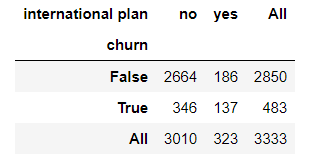
\includegraphics[width=0.7\textwidth]{model1} 
\end{figure}

Accuracy: 0.84\\

precision: 0.885\\

Recall:0.935\\

$\textbf{13}$\\

Given International plan = ‘yes’:\\

False    186
True     137
Name: churn, dtype: int64\\

Given International plan = ‘no’:\\

False    2664
True      346
Name: churn, dtype: int64\\

P(churn = True $ | $ international plan = ‘yes’) = 137/(137+186)=0.424\\

P(churn = False $ | $ international plan = ‘yes’) =
0.576\\

P(churn = True $ | $ international plan = ‘no’) =
0.115\\

P(churn = False $ | $ international plan = ‘no’) =
0.885\\

P(churn = True) = 483/3333 = 0.145\\

P(churn = False) = 1-0.145 = 0.855\\

P(opted $ | $ churn = True) = P(churn = True $ | $ international plan = ‘yes’) * P(international plan = ‘yes’)/P(churn = True) = 0.424 * 0.097/0.145 = 0.284\\

P(not-opted $ | $ churn = True) = P(churn = True $ | $ international plan = ‘no’) * P(international plan = ‘no’)/P(churn = True) = 0.115 * 0.903/0.145 = 0.716\\

P(opted $ | $ churn = False) = P(churn = False $ | $ international plan = ‘yes’) * P(international plan = ‘yes’)/P(churn = False) = 0.576 * 0.097/0.855 = 0.065\\

P(not-opted $ | $ churn = False) = P(churn = False $ | $ international plan = ‘no’) * P(international plan = ‘no’)/P(churn = False) = 0.885 * 0.903/0.855 = 0.935\\

$\textbf{14}$\\

Given that the customer has opted for an international plan, the chances of the customer staying with the company:0.424\\

Given that the customer has opted for an international plan, the chances of the customer not-staying with the company:0.576\\

Given that the customer has not opted for an international plan, the chances of the customer staying with the company:0.115\\

Given that the customer has not opted for an international plan, the chances of the customer not-staying with the company: 0.885\\

When the customer has opted for an international plan, the chance of staying the company or not would be similar. But when the customer has not opted for an international plan, they are tend to churn the company.\\

$\textbf{15}$\\

[0.13199426111908177, 0.10330228619813717, 0.11462450592885376, 0.10256410256410256, 0.4578313253012048, 0.6060606060606061, 0.6363636363636364, 0.5555555555555556, 0.5, 1.0]. These are the probability of customers leaving the company given the number of customer service call he made(from 0 to 9).\\
 
\begin{figure}[H] 
\centering 
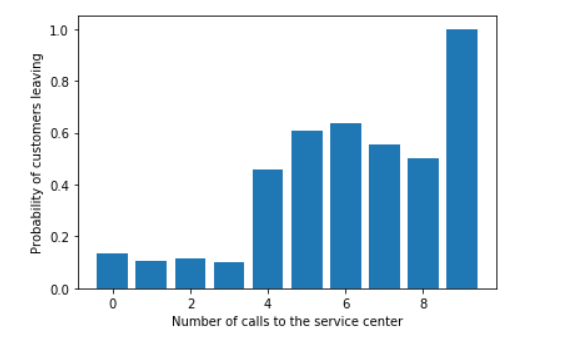
\includegraphics[width=0.7\textwidth]{prob} 
\end{figure}

The probabilities of a customer leaving the company given number(from 0 to 3) of calls to the service center are similar and The probabilities of a customer leaving the company given number(from 4 to 8) of calls to the service center are similar.\\

By comparing the data, we could find that the probability of a customer leaving the company given low number of calls to the service center is low, then the probability increases as the number of calls to the service center increases and it reaches 1 when the number of calls to the service center reaches 9.\\

$\textbf{16}$\\

\begin{figure}[H] 
\centering 
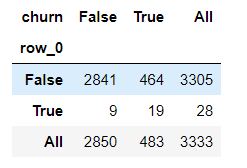
\includegraphics[width=0.7\textwidth]{last} 
\end{figure}

Accuracy = 0.855\\

precision = 0.997\\

recall = 0.86\\

\newpage

$\textbf{Problem 2}$\\

$\textbf{1}$\\

\begin{figure}[H] 
\centering 
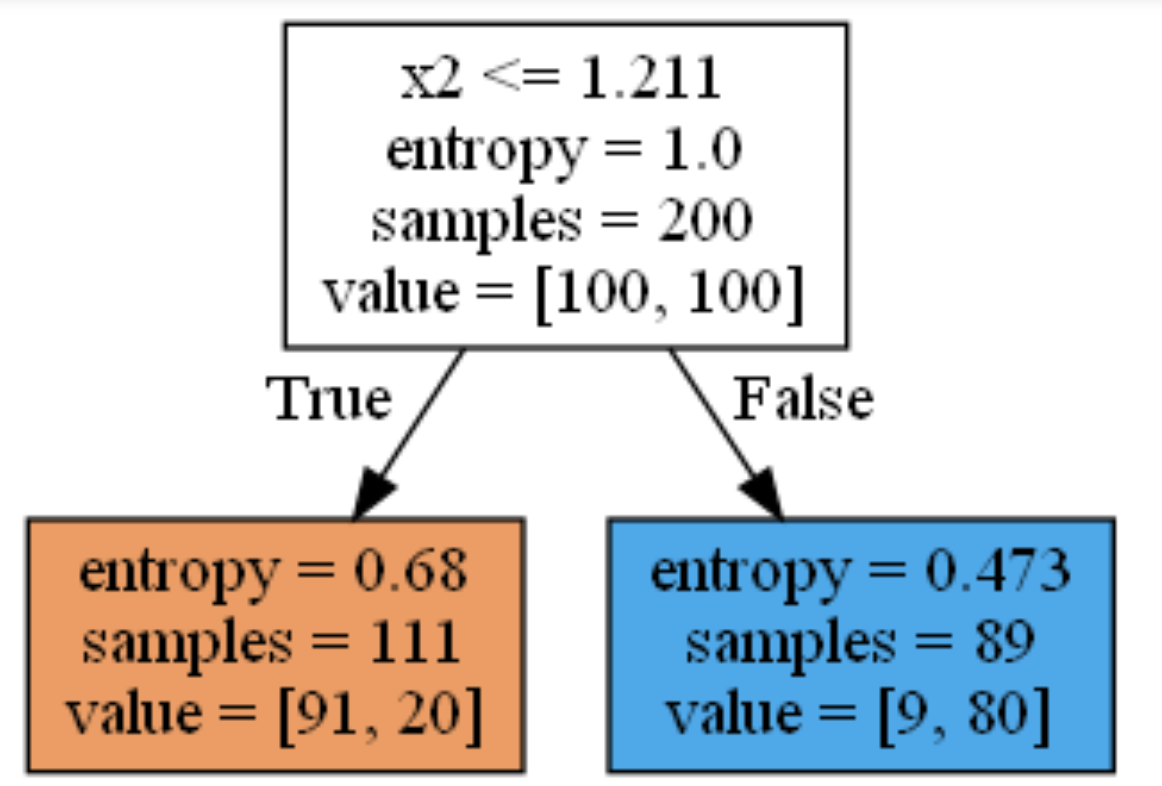
\includegraphics[width=0.7\textwidth]{decisiontree1} 
\caption{Decision Tree for max depth = 1}
\end{figure}

\begin{figure}[H] 
\centering 
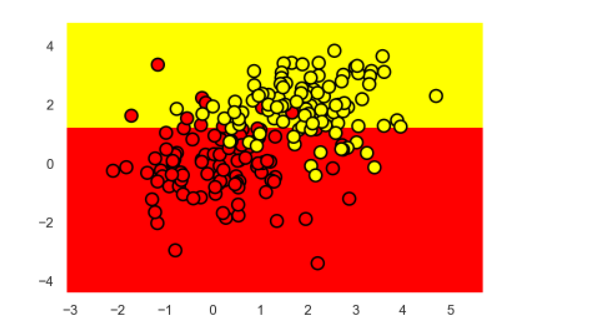
\includegraphics[width=0.7\textwidth]{decisionboundary1} 
\caption{Decision Tree Boundary for max depth = 1}
\end{figure}

\begin{figure}[H] 
\centering 
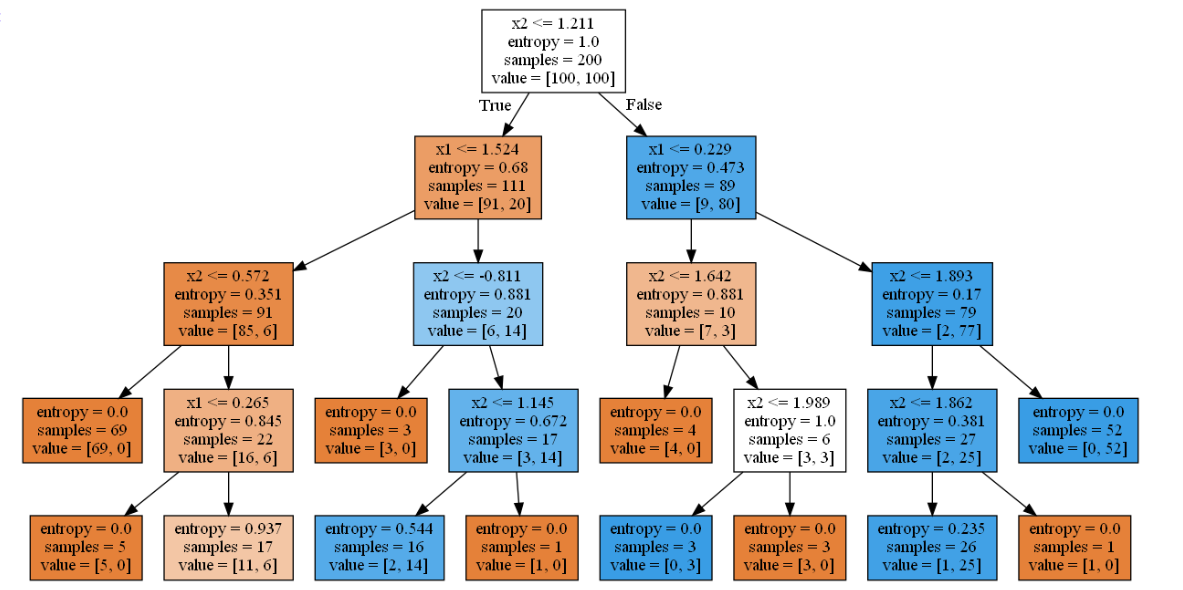
\includegraphics[width=0.7\textwidth]{decisiontree4} 
\caption{Decision Tree for max depth = 4}
\end{figure}

\begin{figure}[H] 
\centering 
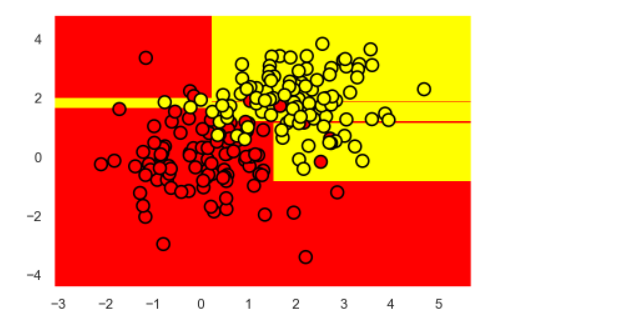
\includegraphics[width=0.7\textwidth]{decisionboundary4} 
\caption{Decision Tree Boundary for max depth = 4}
\end{figure}

$\textbf{2}$\\

For max depth, if the parameter is not specified, the nodes are expanded until all leaves are pure.\\

For criterion, the default value would be "gini"\\

$\textbf{3}$\\

5 different age values: 43.5,19.0,22.5,30.0,32.0\\

They are the mean values between the ages of switching between 1 and 0.\\

For example, 19 is the mean value of 18 and 20.\\

$\textbf{4}$\\

The idea of kNN method is: Given a training data set, for a new input instance, find the K instances (that is, the K neighbors mentioned above) closest to the instance in the training data set. If most of these K instances belong to a certain class, the input instance is classified into this class.\\

K is important because it determines the size and shape of the boundary, which will directly affect the accuracy of the kNN algorithm.\\

Default matrix is minkowski matrix. The formula of minkowski matrix is $sum(|x - y|^p)^{1/p}$. For example, when p = 1, it is Hamming distance and when p = 2, it is Euclidean distance.\\

$\textbf{5}$\\

Sometimes, the model trained from the training set performs well on the training set, but the testing results on the testing data are poor, which indicates that the model may have overfitting problem and the generalization performance on unknown data is poor. Cross-validation can make full use of all training data for evaluating and selecting the model.\\

$\textbf{6}$\\

When we leave the value of max depth to its default value, the accuracy would fall. If the max depth is not specified, the nodes
would expanded until all leaves are pure.Thus, the decisiontreeclassifier
would get better performance on the training set but pool generalization 
performance on the testing set.\\

$\textbf{7}$\\

GridSearchCV processes the data column from 1 to m by subtract the mean of current column(column i,where i = 1..m) from each element in the current column and then devided by the standard deviation of the current column.This process is the standardization of the dataset.\\

Scaler transformation: [[-1,-1],[-1,-1],[1,1],[1,1]]\\

$\textbf{8}$\\

GridSearchCV can automatically adjust parameters and then do the cross-validation.As long as the parameters are entered, you can get the most optimized results and parameters.In the example, we can see that we are trying to find the optimal max depth and max features among 1 to 11 and 4 to 19 respectively.The optimal results would be 6 and 17 for max depth and max features repectively.\\

It is important because GridSearchCV() function can be very simple to achieve cross-validation and verify the performance of the calculation model, and then chooses the best combination of parameters for the k-nearest neighbors and decision trees.We can easily avoid the overfitting and underfitting problem.\\

$\textbf{9}$\\

The number of max depth = 9 and the number of max features = 14, so we need to construct 14*9 = 126 decision trees.If we process the 10-fold cross-validation, we need to construct 126*10 = 1260 decision trees.\\


$\textbf{10}$\\

The best choice of k is 9 in the 10-fold cross-validation scenario and the accuracy would be 0.8868.\\

$\textbf{11}$\\

The accuracy of the decision tree [max depth = 5] = 0.667.\\

The accuracy of the K-nearest neighbor [K = 10] = 0.976.\\

The best parameters for holdout
dataset for decision trees are max depth = 10 and max features = 50. The best accuracy would be 0.8426.\\

\newpage

$\textbf{Problem 3}$\\

$\textbf{1}$\\

There are 5572 records. The distribution of the “label” class would be:
ham     4825
spam     747
Name: label, dtype: int64\\

Ham are much more than spam, thus it is skewed.\\

$\textbf{2}$\\

From the describe() method, we can find that there are 5169 unique SMS.\\

The 'Sorry, I'll call later' would be the most frequent SMS and the frequency would be 30.\\

$\textbf{3}$\\

The maximum length of SMS present in the dataset: 910\\

The minimum length of SMS present in the dataset: 2\\

\begin{figure}[H] 
\centering 
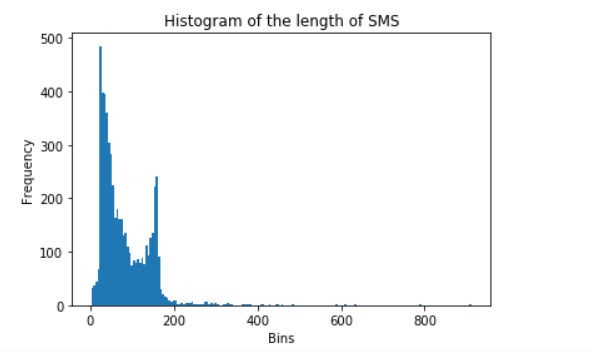
\includegraphics[width=0.7\textwidth]{histogram1} 
\caption{Bin Size = 5}
\end{figure}

\begin{figure}[H] 
\centering 
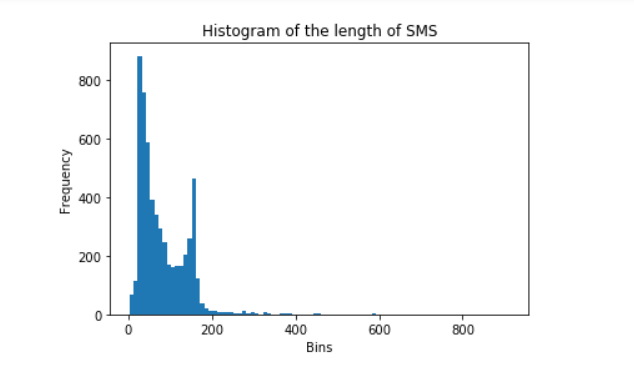
\includegraphics[width=0.7\textwidth]{histogram2} 
\caption{Bin Size = 10}
\end{figure}

\begin{figure}[H] 
\centering 
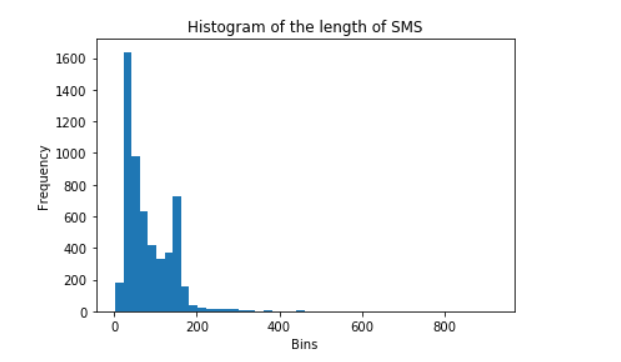
\includegraphics[width=0.7\textwidth]{histogram3} 
\caption{Bin Size = 20}
\end{figure}

\begin{figure}[H] 
\centering 
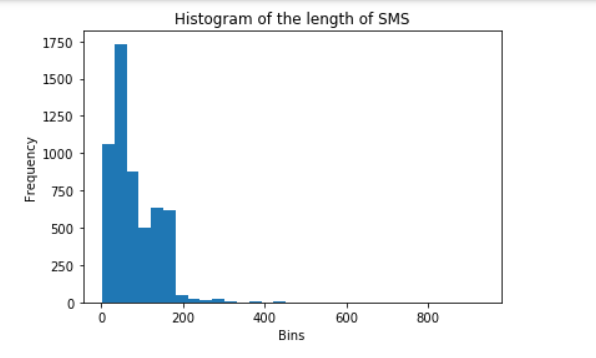
\includegraphics[width=0.7\textwidth]{histogram4} 
\caption{Bin Size = 30}
\end{figure}

\begin{figure}[H] 
\centering 
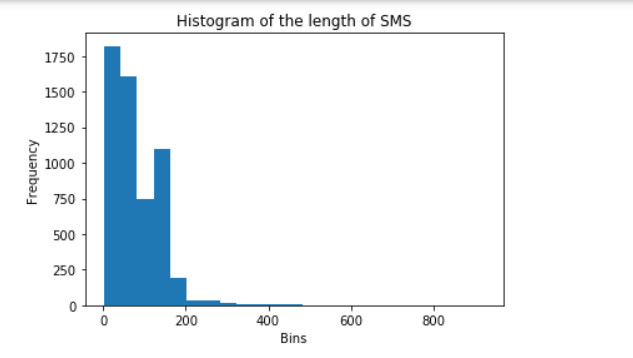
\includegraphics[width=0.7\textwidth]{histogram5} 
\caption{Bin Size = 40}
\end{figure}

\begin{figure}[H] 
\centering 
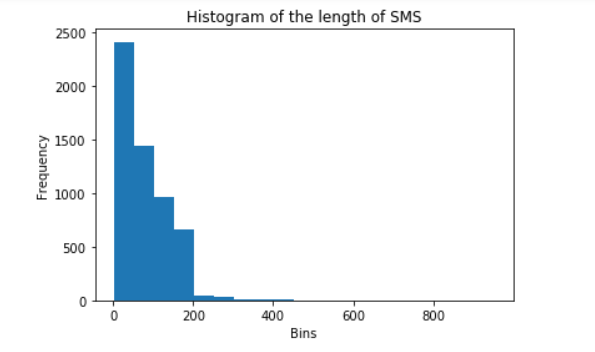
\includegraphics[width=0.7\textwidth]{histogram6} 
\caption{Bin Size = 50}
\end{figure}

\begin{figure}[H] 
\centering 
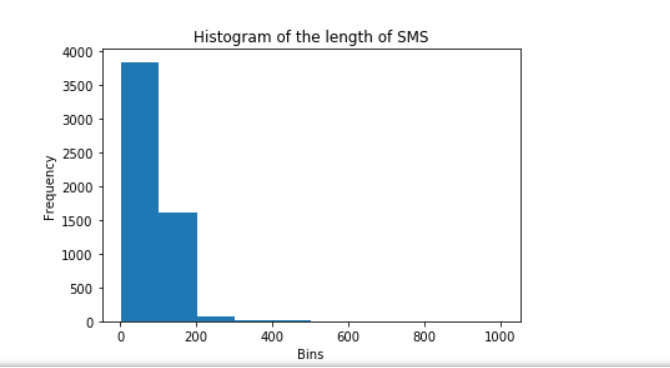
\includegraphics[width=0.7\textwidth]{histogram7} 
\caption{Bin Size = 100}
\end{figure}

\begin{figure}[H] 
\centering 
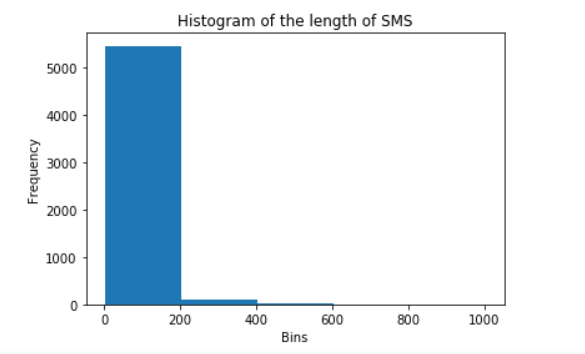
\includegraphics[width=0.7\textwidth]{histogram8} 
\caption{Bin Size = 200}
\end{figure}


We assume the samples follow Gaussian Distribution and each sample is independent.\\

$\textbf{4}$\\

\begin{figure}[H] 
\centering 
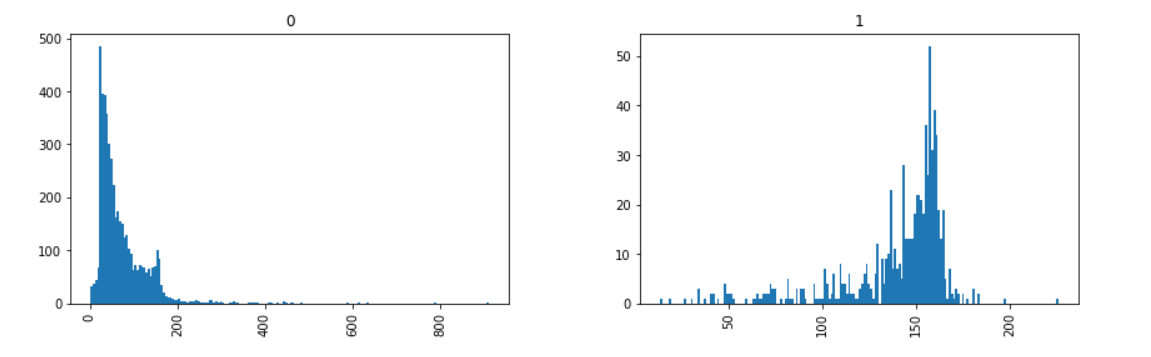
\includegraphics[width=0.7\textwidth]{SMS1} 
\caption{Bin Size = 5}
\end{figure}

\begin{figure}[H] 
\centering 
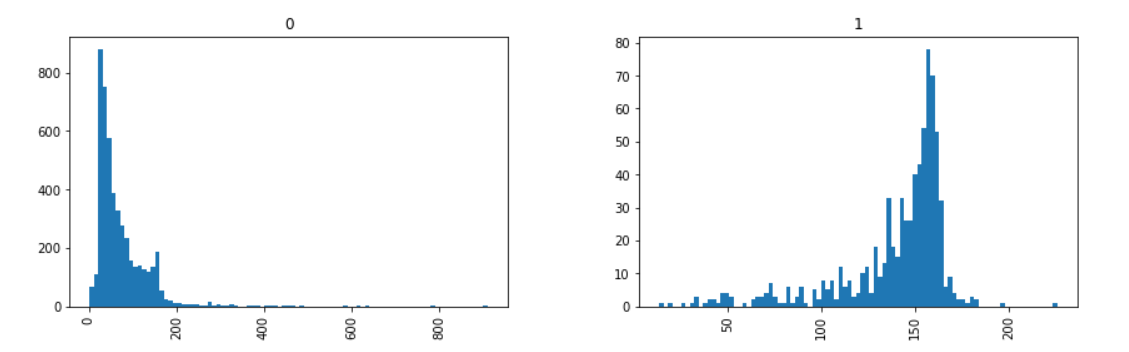
\includegraphics[width=0.7\textwidth]{SMS2} 
\caption{Bin Size = 10}
\end{figure}

\begin{figure}[H] 
\centering 
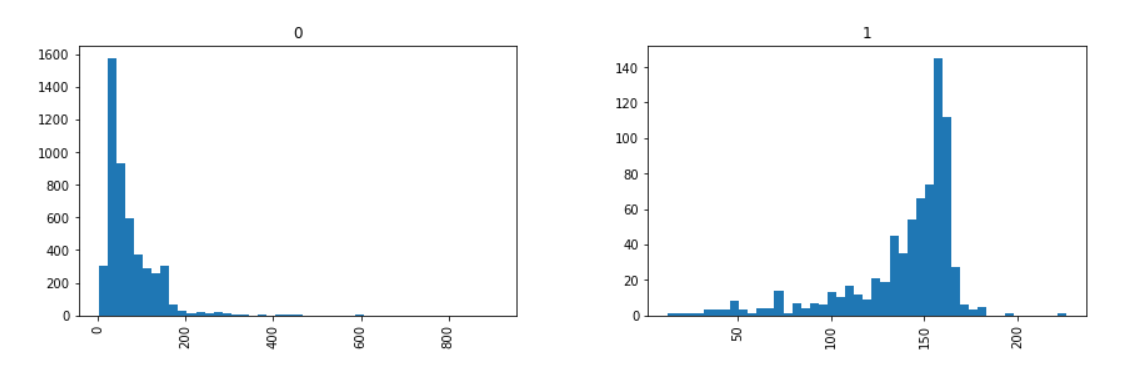
\includegraphics[width=0.7\textwidth]{SMS3} 
\caption{Bin Size = 20}
\end{figure}

\begin{figure}[H] 
\centering 
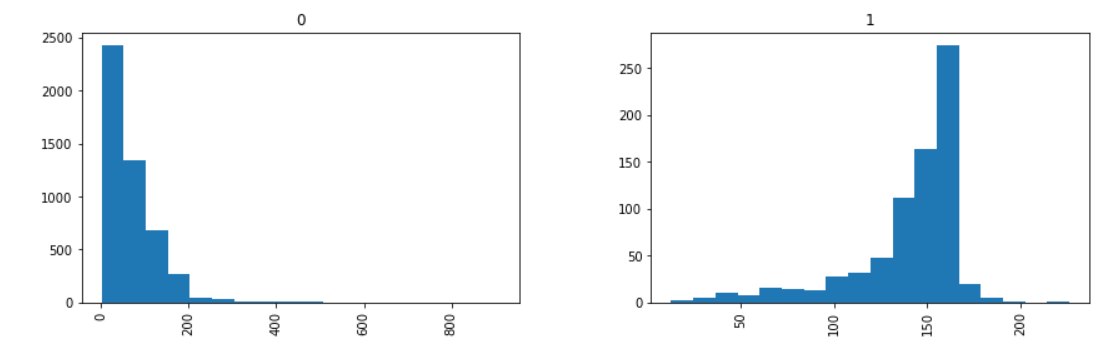
\includegraphics[width=0.7\textwidth]{SMS4} 
\caption{Bin Size = 50}
\end{figure}

The shape for each histogram of the length of SMS for each label remains the same for the most part. But when bin size is increasing, the bars of the histogram are getting thicker and the shape becomes more and more rough, which is reasonable.

$\textbf{5}$\\

Under the Bag of words, a piece of text (which may be a sentence or a document) can be represented by a bag containing these words and the  representation does not consider the grammar and the order of the words. \\

Assume we have thousands of books, the length of the generated vector at this time may be as long as tens of thousands, and for each book may only contain a few words in the dictionary, so that for each book The vector generated by the book will contain a large number of zeros. Such a vector becomes a sparse vector or sparse representation. So we need to convert all strings into lower cases to decrease the size of the vector.\\

Convert all strings into the upper case would also fulfill our original goal.\\

$\textbf{6}$\\

CountVectorizer() method is using to clean our data, it could convert all words to lower case and remove punctuation marks.\\

If we set set stop words = 'english',the CountVectorizer would give us the English step word from the input, which fits the step word list defined in sk-learn.\\

Five examples of stop-words in English: fine,ok,test,thank,tomorrow.\\

$\textbf{7}$\\

We first seperate the data into train/test set and then generate the document-term matrix for each set. The reason is that if we do not seperate the data before generate the document-term matrix, the test set data would change the frequency of the word and affect the model generate from the train set.\\

$\textbf{8}$\\

Document-term matrix:\\

\begin{figure}[H] 
\centering 
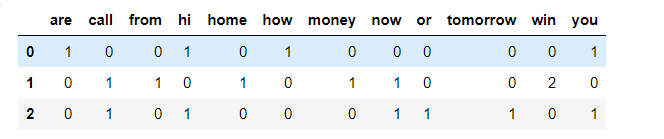
\includegraphics[width=0.7\textwidth]{documentterm} 
\caption{Document Term Matrix}
\end{figure}

$\textbf{9}$\\

7777 features are created while making document-term matrix for SMS dataset.

After tokenizing the words, we could do the stemming to reduce the feature of the document-term matrix.Stemming is the process of removing the prefix and suffix of a word and getting the root. For example, friendly and friends in the text mean similar, and can be regarded as one word(friend)and then put the stem into the word bag.\\

Stemming can reduce the number of features. But some information would be lost since the meaning between words would not be 100 percentages the same. For example, friendly and friends, although these two words in the text mean similar, they are a little bit different.\\

$\textbf{10}$\\

We should use Multinomial Naive Bayes because it would treat the word counts as input and consider the term frequency, which means it is suitable for discrete input. Gaussian Naive Bayes would treat the input data has a Gaussian distribution and it is better for continuous data.\\

Accuracy score: 0.9847533632286996\\

Precision score: 0.9420289855072463\\

Recall score: 0.935251798561151\\

F1 score: 0.9386281588447652\\

\newpage

$\textbf{Problem 4}$\\

For Diabetes data, the dimension would be 768*9. The outcome is not balance, which we have 500 samples for health people and 268 samples for the people who have Diabetes. After plotting the graphs, we can find that BMI, BloodPressure and Glucose attributes follow the normal distribution while other attributes follow the exponential distribution.After cleaning the data, we processed KNN, DecisionTree, Gaussian Naive Bayes and Bernoulli Naive Bayes for this data set and the final accuracies would be 0.714136,0.686720,0.754205 and 0.656069, respectively. The Gaussian Naive Bayes has the highest accuracy. These results are very interesting that all of them are not good. There are two explanations for this phenomenon.The first one is that the Diabetes data set is not linearly separable in the low dimension,which means we need to map the data to high dimensions and then find the hyperplane.We could use SVM with rbf kernel or poly kernel.The second one is that this data set itself is not good, which means it cannot be distinguished well by using machine learning technique.\\

For Iris data, the dimension would be 150*5. After plotting the graphs, we can find that all attributes follow the normal distribution. After cleaning the data, we processed the KNN, DecisionTree, Bernoulli Naive Bayes and Gaussian Naive Bayes for this data set and the final accuracies would be 0.966667,0.960000,0.333333 and 0.953333, respectively. The kNN has the highest accuracy. For this data set, four algorithms besides Bernoulli Naive Bayes have good performance. There is an interesting result that the accuracy of Gaussian Naive Bayes is much higher than that of the Bernoulli Naive Bayes. The reason would be the distribution of data. Since all the attributes follow the normal distribution, it is reasonable that the Bernoulli Naive Bayes performs poorly.\\

For thyroid data,the dimension would be 215*6. After plotting the graphs, we can find that Serum thyroxin and T3 resin follow the normal distribution and other attributes do not follow any distribution. Then, we processed the KNN, DecisionTree, Gaussian Naive Bayes and Bernoulli Naive Bayes for this data set and the final accuracies would be 0.925758,0.944156,0.967749 and 0.734848, respectively. The GNB has the highest accuracy. For this data set, four algorithms besides Bernoulli Naive Bayes have good performance. From these three data sets, we can find out that the Bernoulli Naive Bayes is limited.\\

$\textbf{Problem 5}$\\

$\textbf{1}$\\

Accuracy:0.76555\\

Position:Around 14350

\begin{figure}[H] 
\centering 
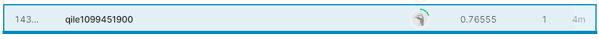
\includegraphics[width=0.7\textwidth]{sc1} 
\end{figure}

$\textbf{2}$\\

Accuracy:0.37799\\

Position:The same as question(1), no improvement.

\begin{figure}[H] 
\centering 
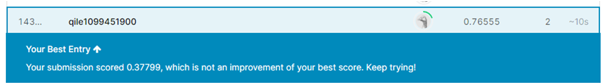
\includegraphics[width=0.7\textwidth]{sc2} 
\end{figure}

$\textbf{3}$\\

Accuracy:0.62200\\

Position:The same as question(1), no improvement.

\begin{figure}[H] 
\centering 

\includegraphics[width=0.7\textwidth]{sc3} 
\end{figure}

$\textbf{4}$\\

Accuracy:0.77511\\

Position:Around 10230

\begin{figure}[H] 
\centering 
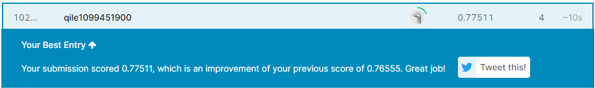
\includegraphics[width=0.7\textwidth]{sc4} 
\end{figure}

$\textbf{5}$\\

Accuracy:0.77751\\

Position:5904

\begin{figure}[H] 
\centering 
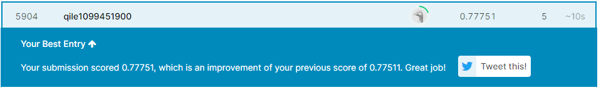
\includegraphics[width=0.7\textwidth]{sc5} 
\end{figure}

\newpage
This kernel teaches us the framework of utilizing machine learning on the data set.\\

First, we need to define the problem and gather the data. The we need to preprocess the data, such as standardizing the data, cleaning the data, deleting irrelevant attributes, dealing with the missing values, converting the data, formatting the data and splitting the dataset to train set and the test set.\\

Next step is Perform Exploratory Analysis. By analyzing the shape, the features and the distribution of the data, we could determine which model we need to process on the dataset. For example, if the data is linear inseparable, we might do not want to use perceptron; if the attributes of the data follow the Gaussian distribution, we might do not want to use Bernoulli Naive Bayes.\\

Next step is Model Data. We use our machine learning algorithm to process data.We would use cross validation and scoring metrics to rank and compare our algorithms’ performance.For example, using decision tree on the thyroid data and using cross validation to select the model.Then, based on the performance of the model, we can try many ways to improve the performance, such as tune model with Hyper-Patameters,  tune model with Feature Selection.\\

Finally, we could validate our model on the validation set and test it on the testing set to see if the model has good generalization performance.If the result is not meeting the expectation, we might need to repeat the previous step.\\ 


\end{document}